\vspace{1cm}
\section{Leitungsgeführte EM-Wellen}
\subsection{Feldtypen im homogenen zylindrischen Wellenleiter}
\begin{itemize}
    \itemsep0pt
    \item Nicht zwingend kreiszylindrisch!
    \item Translationsinvarianz des Wellenleiters in z-Richtung
    \item Ausbreitungskoeffizient $\gamma$:
        \begin{itemize}
            \itemsep0pt
            \item Sich ausbreitende Welle:\\
                \(\gamma = 0 + j\beta,\; q \leq k\)
            \item Evaneszente (gedämpfte) Welle:\\
                \(\gamma = \alpha + j0,\; q > k\)
            %\item Abklingende, sich ausbreitende, Welle: \(\gamma = \alpha + j\beta\)
        \end{itemize}
    \item Modenspezifischer, geometrieabhängiger Eigenwert \(q\):\\
        \(|k|^2 = k_x^2 + k_y^2 + k_z^2 = q^2 + k_z^2,\: k = \omega_c \sqrt{\mu\epsilon}\)
    \item Ausbreitung \textit{nur} oberhalb der Cut-off-Frequenz \(f_c\) bzw. \(\omega_c\) \(\implies k_z = 0\)\\
    \item Feldwellen(typ)-Widerstände:
        \begin{align*}
            Z_{FH} &= \dfrac{j\omega\mu}{\gamma_H} = \dfrac{\omega\mu}{\beta_H} = \dfrac{\lambda_g}{\lambda_{HEW}}Z_{F}\\
            Z_{FE} &= \dfrac{j\omega\mu}{\gamma_E} = \dfrac{\beta_E}{\omega\epsilon} = \dfrac{\lambda_g}{\lambda_{HEW}}Z_{F}\\
            \lambda_g &= \dfrac{2\pi}{\beta} = \dfrac{2\pi}{\sqrt{\omega^2\epsilon\mu - q^2}},\
            Z_F = \sqrt{\dfrac{\mu}{\epsilon}}
        \end{align*}
\end{itemize}
\subsection{Phasen- und Gruppen-Geschwindigkeit}
\begin{itemize}
    \itemsep0pt
    \item Phasengeschwindigkeit: \(v_p = \dfrac{\omega}{\beta}\)
    \item (Gruppen-)Geschwindigkeit der informationstragenden Hüllkurve:\\
        \(v_g = \left( \dfrac{\mathrm{d}\beta}{\mathrm{d}\omega} \right)^{-1}\)
    \item \(\dfrac{v_p}{c_0} =  \dfrac{\lambda_g}{\lambda_0} = \dfrac{Z_{FH}}{Z_0} =\
        \left(\dfrac{v_g}{c_0}\right)^{-1} = \left(\dfrac{Z_{FE}}{Z_0}\right)^{-1} = \dfrac{k}{k_z}\)
\end{itemize}
\subsection{Fünf-Komponenten-Felder (E- und H-Moden)}
\begin{itemize}
    \itemsep0pt
    \item \textbf{Ansatz:} Im zylind. Wellenleiter, können transversale und longitudinale Felder getrennt betrachtet werden
    \item \((u,v)\) sind beliebige krummlinige Koordinaten:
        \begin{align*}
            \vec{E}(u, v, z) &= \left[ \vec{E}_t(u,v) + \vec{e}_z E_z \right]\mathrm{e}^{-\gamma z}\\
            \vec{H}(u, v, z) &= \left[ \vec{H}_t(u,v) + \vec{e}_z H_z \right]\mathrm{e}^{-\gamma z}
        \end{align*}
    \item Die Kenntnis der z-Komponente reicht, um die restlichen 4 Komponenten zu berechnen
\end{itemize}
\subsection{Rechteckhohlleiter}
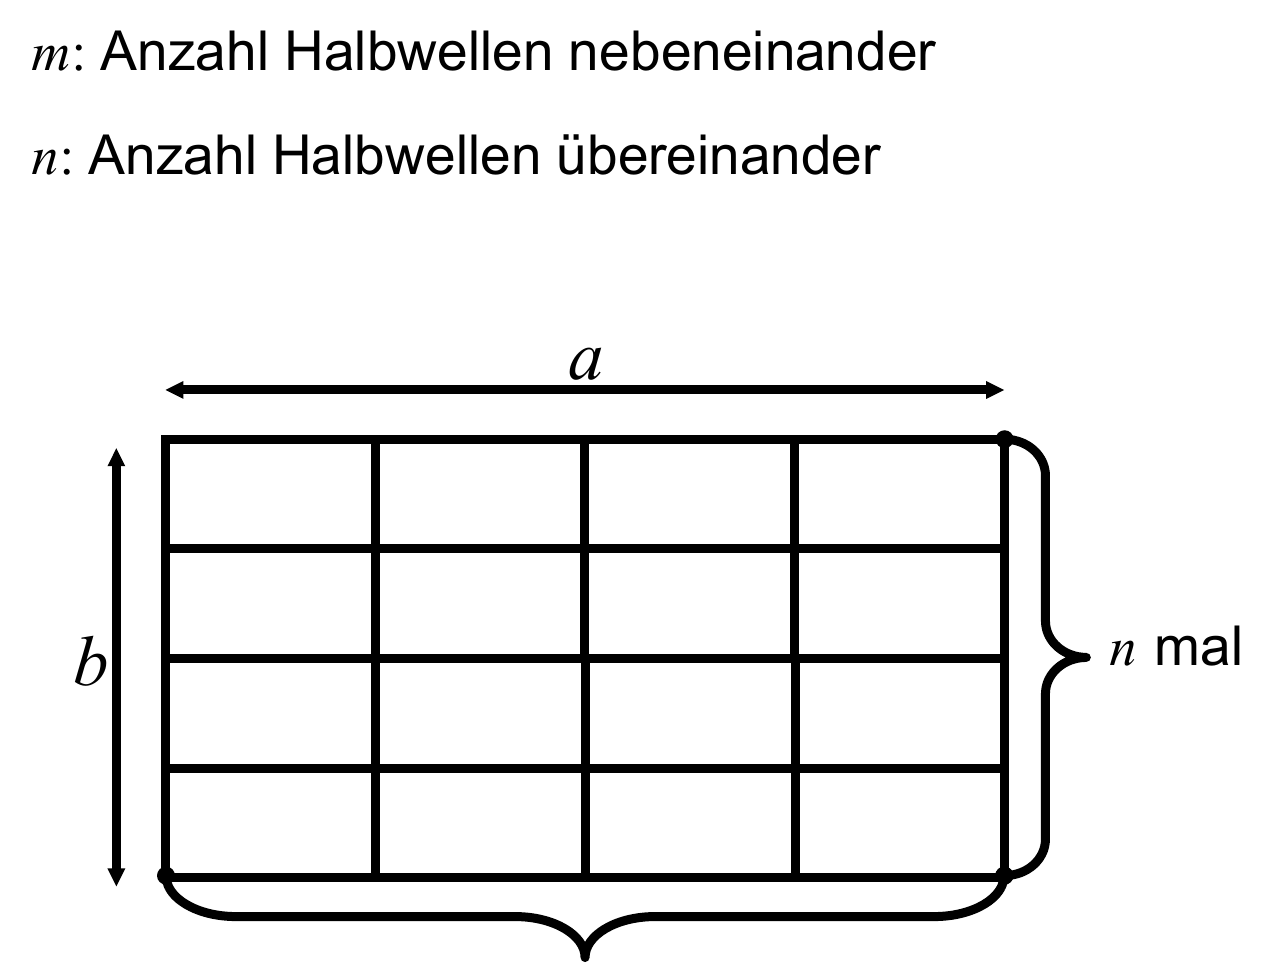
\includegraphics[width=.35\paperheight]{content/fuw/pictures/fuw_rechteckhohlleiter.png}
\begin{itemize}
    \itemsep0pt
    \item \(E_{mn}\) (TM)-Moden/Feldtypen im Rechteckhohlleiter \(H_z = 0\):
        \begin{align*}
            E_z &= E_0 \sin\left(\dfrac{m\pi x}{a}\right)\sin\left(\dfrac{n\pi y}{b}\right)\mathrm{e}^{-j\beta z},\\
            E_y &= -j\dfrac{\beta}{\beta_c^2} \dfrac{m\pi}{a}  E_0\cos\left(\dfrac{m\pi x}{a}\right)\sin\left(\dfrac{n\pi y}{b}\right)\mathrm{e}^{-j\beta z},\\
            E_x &= j\dfrac{\beta}{\beta_c^2} \dfrac{n\pi}{b} E_0 \sin\left(\dfrac{m\pi x}{a}\right)\cos\left(\dfrac{n\pi y}{b}\right)\mathrm{e}^{-j\beta z},\\
            H_y &= -H_x Z_{FH},\\
            H_x &= H_y Z_{FH}
        \end{align*}
    \item \(H_{mn}\) (TE)-Moden/Feldtypen im Rechteckhohlleiter \(E_z = 0\):
        \begin{align*}
            H_z &= H_0 \cos\left(\dfrac{m\pi x}{a}\right)\cos\left(\dfrac{n\pi y}{b}\right)\mathrm{e}^{-j\beta z},\\
            H_y &= j\dfrac{\beta}{\beta_c^2} \dfrac{n\pi}{b}  H_0 \cos\left(\dfrac{m\pi x}{a}\right)\sin\left(\dfrac{n\pi y}{b}\right)\mathrm{e}^{-j\beta z},\\
            H_x &= j\dfrac{\beta}{\beta_c^2} \dfrac{m\pi}{a} H_0 \sin\left(\dfrac{m\pi x}{a}\right)\cos\left(\dfrac{n\pi y}{b}\right)\mathrm{e}^{-j\beta z},\\
            E_y &= -\dfrac{E_y}{Z_{FE}},\\
            E_x &= \dfrac{E_x}{Z_{FE}}
        \end{align*}
    \item Cut-off-Wellenlänge: \(\lambda_c = \dfrac{1}{\sqrt{ \left(\dfrac{m}{2a}\right)^2 + \left(\dfrac{n}{2b}\right)^2 }}\)
    \item \(\beta_c = \dfrac{2\pi}{\lambda_c}\)
\end{itemize}
%\begin{itemize}
%    \item Verlustleistung:
%        \begin{align*}
%            \Delta P_1 &= -\dfrac{1}{4}R_{\Box}a\dfrac{|E_0|^2}{|Z_{FH}|^2}\Delta z\\
%            \Delta P_2 &= -\dfrac{1}{4}R_{\Box}a\dfrac{|E_0|^2}{|Z_{F0}|^2} \left(\dfrac{\lambda_0}{2a}\right)^2 \Delta z\\
%            \Delta P_3 &= \dfrac{1}{2}R_{\Box}b\dfrac{|E_0|^2}{|Z_{F0}|^2} \left(\dfrac{\lambda_0}{2a}\right)^2 \Delta z
%        \end{align*}
%    \item Dämpfungskonstante: \[\alpha = \dfrac{R_{\Box}}{Z_{F0}} \dfrac{\frac{1}{b} + \frac{2}{a} \left(\frac{\lambda_0}{2a}\right)^2}{\sqrt{1 - \left(\frac{\lambda_0}{2a}\right)^2}}\
%        \]
%\end{itemize}
\subsection{Hohlleiter unterhalb der kritischen Frequenz}
\textbf{Exponentielle Dämpfung}
\[\alpha = \dfrac{2\pi}{\lambda_{HEW}} \sqrt{\left(\dfrac{\lambda_{HEW}}{\lambda_c}\right)^2 - 1}\
= \dfrac{2\pi}{\lambda_c} \sqrt{1 - \left(\frac{f}{f_c}\right)^2}\]
\subsection{Dielektrische Wellenleiter}

